\documentclass{journal}[IEEEtran, twocolumn]             % No modificar

% PASO 1. Reemplace "Práctica 1" por el número de la práctica que corresponda
\newcommand{\dochead}{Práctica 3}     

% PASO 2. Reemplace "TÍTULO PRÁCTICA" por el título de la práctica que corresponda.
\newcommand{\docsubhead}{Conversión RF-EC}  

% PASO 3. Reemplace "B1A - 02" por el grupo de la asignatura y el número de su grupo de laboratorio
\newcommand{\teamname}{C1}     

% PASO 4. OPCIONAL: Reemplace "\docsubhead \docsubhead" por el título del documento en caso de requerirse.
\newcommand{\titulo}{\dochead: \docsubhead}      

% PASO 5. Reemplace "31 de diciembre de 2030" por la fecha de su documento
\newcommand{\fecha}{12 de octubre de 2024}      

% To load packages
\usepackage[T1]{fontenc}
\usepackage[utf8]{inputenc} 
\usepackage[spanish]{babel}
\usepackage[letter,left=2.0cm,top=2.0cm,right=2.0cm,bottom=4.0cm]{geometry}
\usepackage{amsmath}
\usepackage{amsfonts}
\usepackage{fancyhdr}
\usepackage{fancyvrb}
\usepackage{listings}
\usepackage{array}
\usepackage{graphicx,color,enumerate}	
\usepackage{multirow} 
\usepackage{multicol}
\usepackage{authblk}
\usepackage{charter}    % Font typeface
\usepackage{titling}
\usepackage{url}
\usepackage{hyperref}
\usepackage{xcolor}
\usepackage{booktabs}

\definecolor{uisgreen}{RGB}{125,194,3}
\definecolor{gray97}{gray}{.97}
\definecolor{gray75}{gray}{.75}
\definecolor{gray45}{gray}{.45}

\setlength{\droptitle}{-1.8cm}
\pagestyle{fancy}

%%% Header definition
\headheight=60pt 						% header height 
\renewcommand{\headrulewidth}{4pt}
\let\oldheadrule\headrule% Copy \headrule into \oldheadrule
\renewcommand{\headrule}{\color{uisgreen}\oldheadrule}

\fancyhead[L]							% left header 
{	\begin{minipage}{2.5cm}
		
\includegraphics[scale=0.3]{./figs/uislogohoriz.png} 
	\end{minipage}	
	\begin{minipage}{5cm}
	    \color{uisgreen}
	    \footnotesize {\textsf{Universidad Industrial de Santander\\ 
				Escuela de Ingenierías Eléctrica, \\
				Electrónica y de Telecomunicaciones	}}	
	\end{minipage}
}
\fancyhead[R] { 							%la "C" indica al centro
	\begin{minipage}{8cm}
	    \color{uisgreen}
	    \begin{flushright}
    	    \small{\textsf{Laboratorio de COMUNICACIONES I (27139)}} \\
            \normalsize{\textsf{\dochead: \textbf{\docsubhead}}} \\
    	    \small{\textsf{Grupo: \textbf{\teamname}}}
	    \end{flushright}
    \end{minipage}
    \begin{minipage}{1.2cm}
		
\includegraphics[width=1.0\textwidth]{./figs/logoE3T.png} 
	\end{minipage}	
}
%%% End header definition

\lstset{ frame=Ltb,
     framerule=0pt,
     aboveskip=0.5cm,
     framextopmargin=3pt,
     framexbottommargin=3pt,
     framexleftmargin=0.4cm,
     framesep=0pt,
     rulesep=.4pt,
     backgroundcolor=\color{gray97},
     rulesepcolor=\color{black},
     %
     stringstyle=\ttfamily\color{red!50!brown},
     showstringspaces = false,
     basicstyle=\small\ttfamily,
     commentstyle=\color{gray45},
     keywordstyle=\color{blue}\bfseries,
     %
     numbers=left,
     numbersep=15pt,
     numberstyle=\tiny,
     numberfirstline = false,
     breaklines=true,
   }

% minimizar fragmentado de listados
\lstnewenvironment{listing}[1][]
   {\lstset{#1}\pagebreak[0]}{\pagebreak[0]}

\lstdefinestyle{consola}
   {basicstyle=\scriptsize\bf\ttfamily,
    backgroundcolor=\color{gray75},
   }

\lstdefinestyle{C}
   {language=C,}             % No modificar


\begin{document}                    % No modificar

\title{\textbf{\titulo}}            % No modificar

% PASO 6. Agregar aquí el nombre y código de los autores.  
\author{
Carlos Alberto Cetina - 2215583\\
Brayan Julian Niño Hurtado - 2172301\\
Sergio Camilo Santos - 2172315\\
\href{https://github.com/scsantosdth/CommunicationsII_2024_2_scb.git}{https://github.com/scsantosdth/CommunicationsII_2024_2_scb.git}
}

\affil{\small{Escuela de Ingenierías Eléctrica, Electrónica y de Telecomunicaciones} \\ % No modificar
\small{Universidad Industrial de Santander}} % No modificar

\date{\fecha}                       % No modificar

\maketitle                          % No modificar
\thispagestyle{fancy}          % No modificar

%---------------------------------------------------------------
% PASO 7. **..**...****INICIE SU DOCUMENTO DESDE AQUI***...**...
%%%%% A PARTIR DE AQUÍ EDITE EL DOCUMENTO PARA AGREGAR TODO EL CONTENIDO REQUERIDO PARA EL ENTREGABLE CORRESPONDIENTE
%%%%  Todo el contenido a partir de este punto es SOLAMENTE ILUSTRATIVO.
%
% Para sus imformes, BORRE TODO el contenido de aquí en adelante  EXCEPTO la última línea que contiene el comando: \end{document}


\color{black}

\begin{multicols}{2}

\begin{abstract}
This report analyzes the processing of radio frequency (RF) signals using their conversion to complex envelope (CE) to facilitate modulation and demodulation. Through GNURadio, functional blocks are employed to generate and process RF signals, demonstrating their application in digital communication systems.    
\end{abstract}

\section{Introducción}
  El procesamiento de señales de radiofrecuencia (RF) puede ser complejo, pero el uso de la envolvente compleja (EC) simplifica su análisis y detección de eventos importantes como picos de amplitud o cambios abruptos. Este informe utiliza GNURadio para convertir señales de RF a su forma en EC, mostrando las ventajas de esta técnica en la optimización del procesamiento de señales.


\section{Metodología}

\subsection{Parte A: Comprobar el funcionamiento del frujograma}
Se verificó el correcto funcionamiento del flujograma propuesto para la práctica, utilizando una señal OOK (On-Off Keying) tanto en su versión de radiofrecuencia (RF) como en su representación de envolvente compleja (EC) en banda base. Se hizo el analisis en el dominio del tiempo y frecuencia, comparando las señales moduladas RF y EC. Ademas, se repitieron las observaciones variando la frecuencia de la portadora. \cite{flujgrama}

\subsection{Parte B: Comprender los bloques 'e\_RF\_VCO\_ff' y 'e\_EC\_VCO\_fc'}
Para comprender los bloques 'e\_RF\_VCO\_ff' y 'e\_EC\_VCO\_fc', se comenzó abriendo cada uno en el entorno de GNURadio y seleccionando la opción "Open in Editor" para examinar su código Python. Se modificaron los comentarios de ayuda (help) en inglés para ofrecer una explicación más detallada sobre sus parametros, entradas, salidas y operación.

\subsection{Parte C: Modulación BPSK versión RF y EC}

Para implementar la modulación BPSK en versiones RF y EC, se adaptó el flujograma inicial, activando bloques desactivados y estableciendo las interconexiones necesarias para implementar la modulación BPSK en versiones RF y EC. Y se realizaron pruebas similares a las del punto 1, aplicadas a la modulación BPSK.

\subsection{Parte D: Modulación FSK versión RF y EC y constelación}
Se configuró el flujograma para implementar la modulación FSK en RF y EC guardado como \texttt{RF\_EC\_fsk.grc}, realizando pruebas con variaciones en la frecuencia portadora y la desviación de frecuencias. Se analizaron las señales moduladas en los dominios del tiempo y la frecuencia.

\subsection{Parte E: Preguntas de control}
Preguntas de auto control sobre el flujograma randombinayrectsignal.grc
    
\section{Resultados}
\subsection{Parte A: Comprobar el funcionamiento del frujograma}


En el dominio del tiempo  ({Figura 1), se observó que la señal RF modulada (señal roja) sigue un comportamiento On-Off Keying (OOK) y se observó el incremento el número de ciclos de la señal sinusoidal cuando está activa.\cite{OOK}


    \begin{center}
    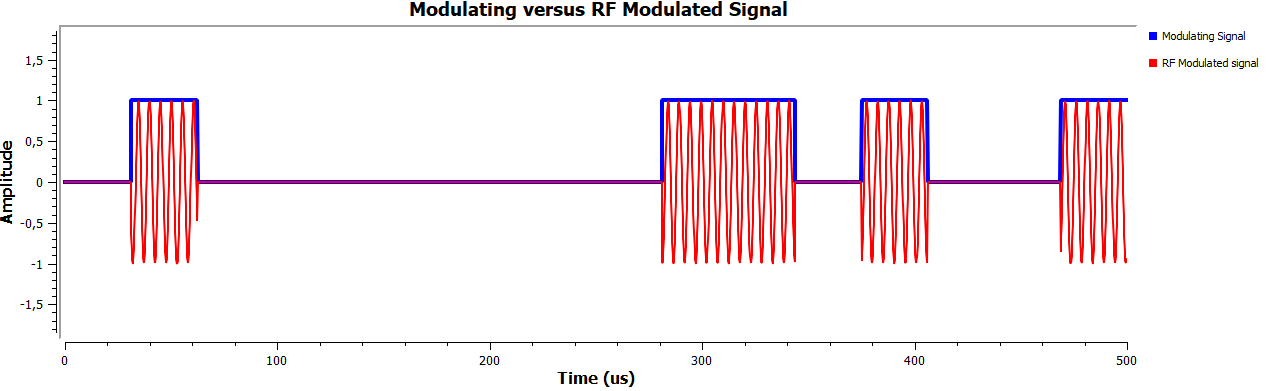
\includegraphics[width=0.45\textwidth]{figs/F1.png}
    \caption{Figura 1: Gráfica en tiempo RF modulada en OOK}
    \label{fig:1}
    \end{center}



Además, en la representación de envolvente compleja (EC)({Figura 2}), la componente 'I' es igual de la señal moduladora, mientras que la componente "Q" siempre es cero, ya que no hay información en cuadratura en la modulación OOK. 

    \begin{center}
    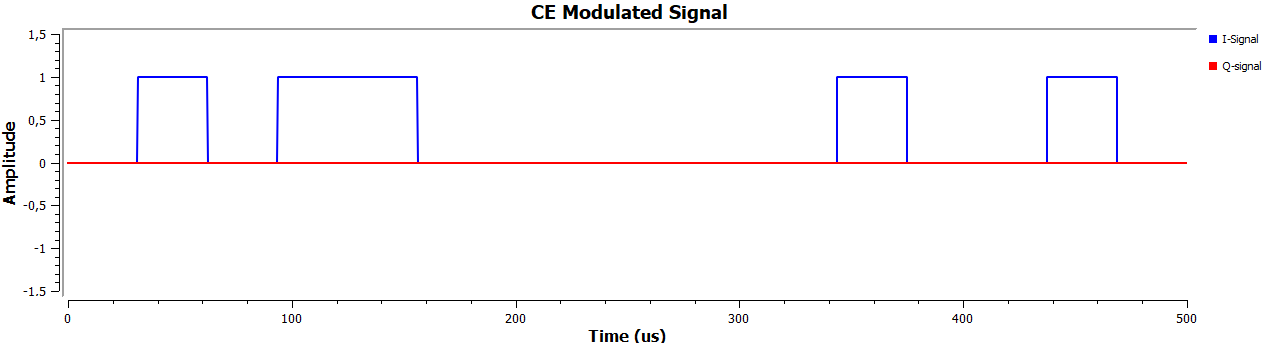
\includegraphics[width=0.45\textwidth]{figs/F2.png}
    \caption{Figura 2: Gráfica en tiempo EC modulada en OOK}
    \label{fig:2}
    \end{center}

En el dominio de la frecuencia, al modular la señal de control de amplitud (EC) con una portadora sinusoidal, se observó que la PSD de la señal modulada se desplazó hacia las frecuencias de la portadora. Este desplazamiento ocurrió debido a que la modulación OOK desplazó el contenido espectral de la señal de banda base hacia dos nuevas bandas, una centrada en la frecuencia positiva de la portadora y otra simétricamente en la frecuencia negativa. Como resultado, la PSD de la señal modulada presentó dos picos, uno en la frecuencia positiva y otro en la negativa de la portadora, replicando así la PSD de la señal EC en ambas bandas.

     \begin{center}
        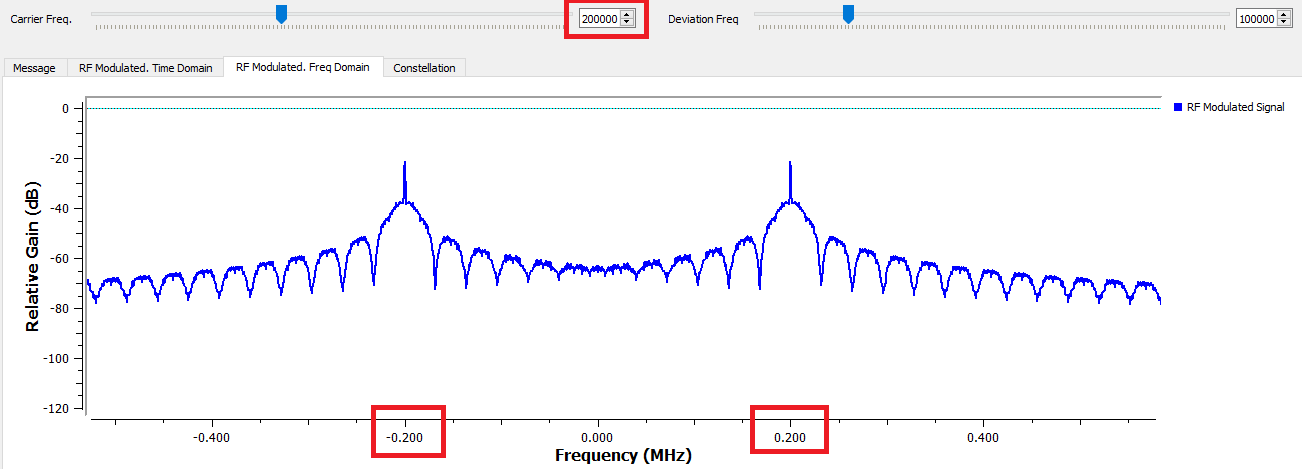
\includegraphics[width=0.45\textwidth]{figs/F3.png}
        \caption{Figura 3: PSD de la señal RF modulada}
        \label{fig:3}
    \end{center}

En el caso de la EC como se observó en la figura 4, que el espectro se concentra alrededor de la frecuencia cero, lo que refleja que la señal está en banda base y no está afectada por la portadora.

    \begin{center}
        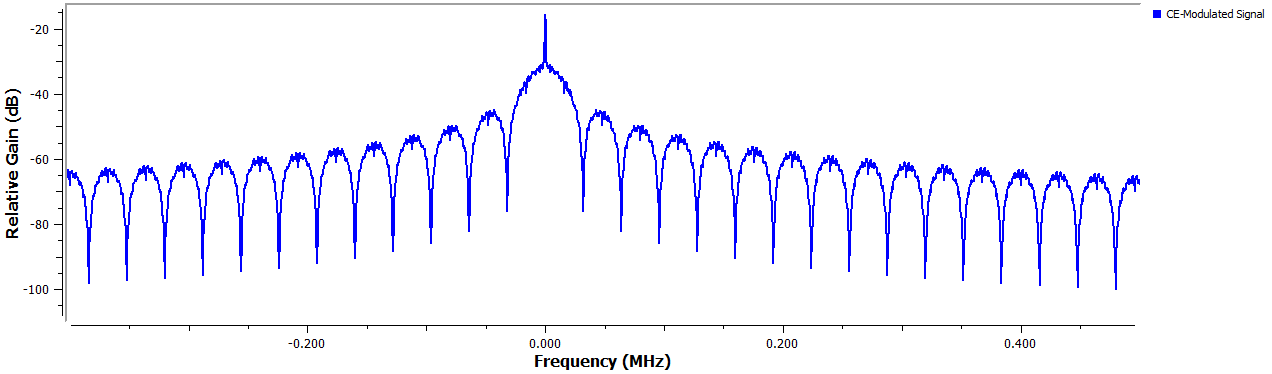
\includegraphics[width=0.45\textwidth]{figs/F4.png}
        \caption{Figura 4: PSD de la EC modulada en OOK}
        \label{fig:4}
    \end{center}
   
  
\subsection{Parte B: Comprender los bloques 'e\_RF\_VCO\_ff' y 'e\_EC\_VCO\_fc'}

\begin{itemize}
 
   \item Boque: 'e\_RF\_VCO\_ff'

This block is an RF VCO that generates a sinusoidal signal.

The parameters include \textit{fc} (Carrier Frequency), setting the oscillator's base frequency at a default of 128 kHz, and \textit{samp\_rate} defines the number of samples per second used by the system, defaulting to 320 kHz.
  
The first input, \textit{A}, controls the output signal's amplitude. The second input, \textit{Q}, modulates the phase. The output is a sinusoidal signal, with amplitude determined by \textit{A} and phase by \textit{Q}, and its frequency is based on \textit{fc} and the phase shift \textit{Q}.

    \item Boque: 'e\_EC\_VCO\_fc'

This block is a CE Voltage-Controlled Oscillator (VCO), or baseband VCO, and works as follows: it generates a complex sinusoidal signal based on the input signals. 

the first input, \textit{A}, which controls the amplitude of the output signal, and the second input, \textit{Q}, modulates the phase of the generated signal. The output is a complex-valued signal, where the real part corresponds to the in-phase component and the imaginary part to the quadrature component.
 
\end{itemize}

\subsection{Parte C: Modulación BPSK versión RF y EC}

Como se observa en la figura 5 a señal modulada en RF es una portadora sinusoidal cuya fase cambia en función de la modulating signal. Un nivel alto mantiene la fase original de la portadora, mientras que un nivel bajo cambia la fase dependiendo de la posición en el diagrama de constelación. Esto genera una señal continua donde cada bit de la señal moduladora corresponde a un estado de fase definido.

 \begin{center}
        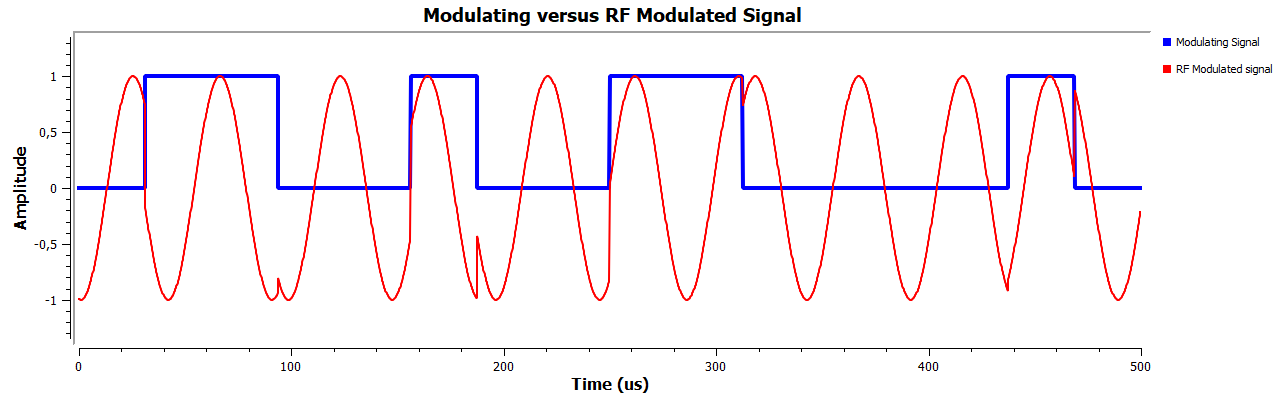
\includegraphics[width=0.45\textwidth]{figs/F5.png}
        \caption{Figura 5: Gráfica en tiempo RF modulada en BPSK}
        \label{fig:5}
    \end{center}
    
    
En la figura 6 de la señal EC modulated signal, se observa que la componente I (real) alterna entre los valores 0.5 y 1, mientras que la componente Q (imaginaria) varía entre 0.8 y 0. Esto corresponde a los puntos de la constelación ubicados en (0.5, 0.8) y (1, 0), reflejando la modulación BPSK en el plano complejo. La señal I tiene una forma escalonada que representa cambios en la amplitud según los bits transmitidos, mientras que la señal Q también exhibe una forma escalonada, indicando la variación de fase asociada.


 \begin{center}
        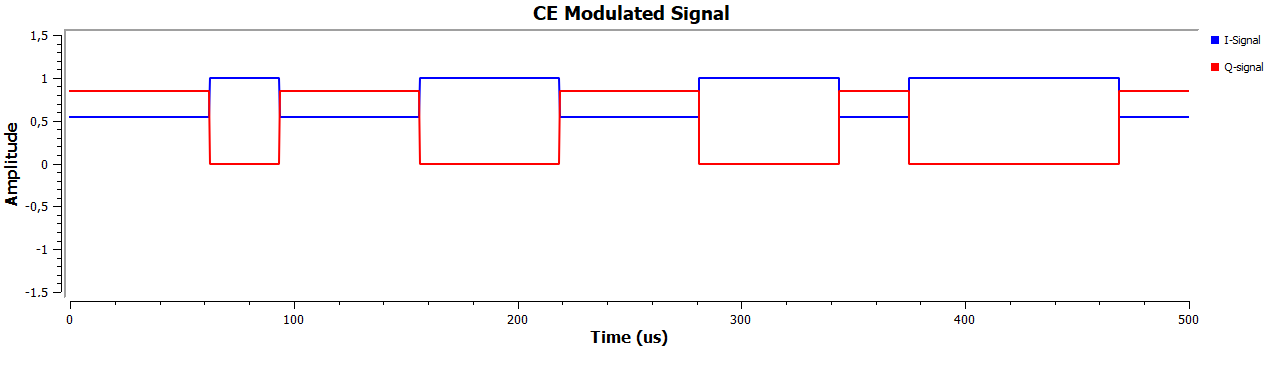
\includegraphics[width=0.45\textwidth]{figs/F6.png}
        \caption{Figura 6: Gráfica en tiempo EC en BPSK}
        \label{fig:6}
    \end{center}
    
La diferencia clave entre BPSK en versión RF y EC es que, en RF, solo se modula la fase de la portadora, mientras que en EC se modulan tanto la fase como la amplitud.\cite{libro1}


\subsection{Parte D: Modulación FSK versión RF y EC y constelación}

\paragraph{Resumen del flujo general:}
En este proceso, la señal original se genera como un flujo de valores aleatorios, que se transforma gradualmente mediante escalado, interpolación y acumulación. Finalmente, se obtiene la modulación FSK en dos versiones: RF (Radio Frecuencia) y EC (Banda Base Compleja). Los bloques \texttt{Virtual Sink} permiten monitorear y analizar cada etapa del flujo.
\paragraph{Comportamiento de la señal modulada:}
En la figura 7 se puede observar la seña modulada en version RF y EC con una frecuencia portadora constante de 128000 Hz y una desviaciónde frecuencia de 32000 Hz que seran los valores de frecuencias constantes que se utilizaran para hacer las siguientes variaciones.
 \begin{center}
        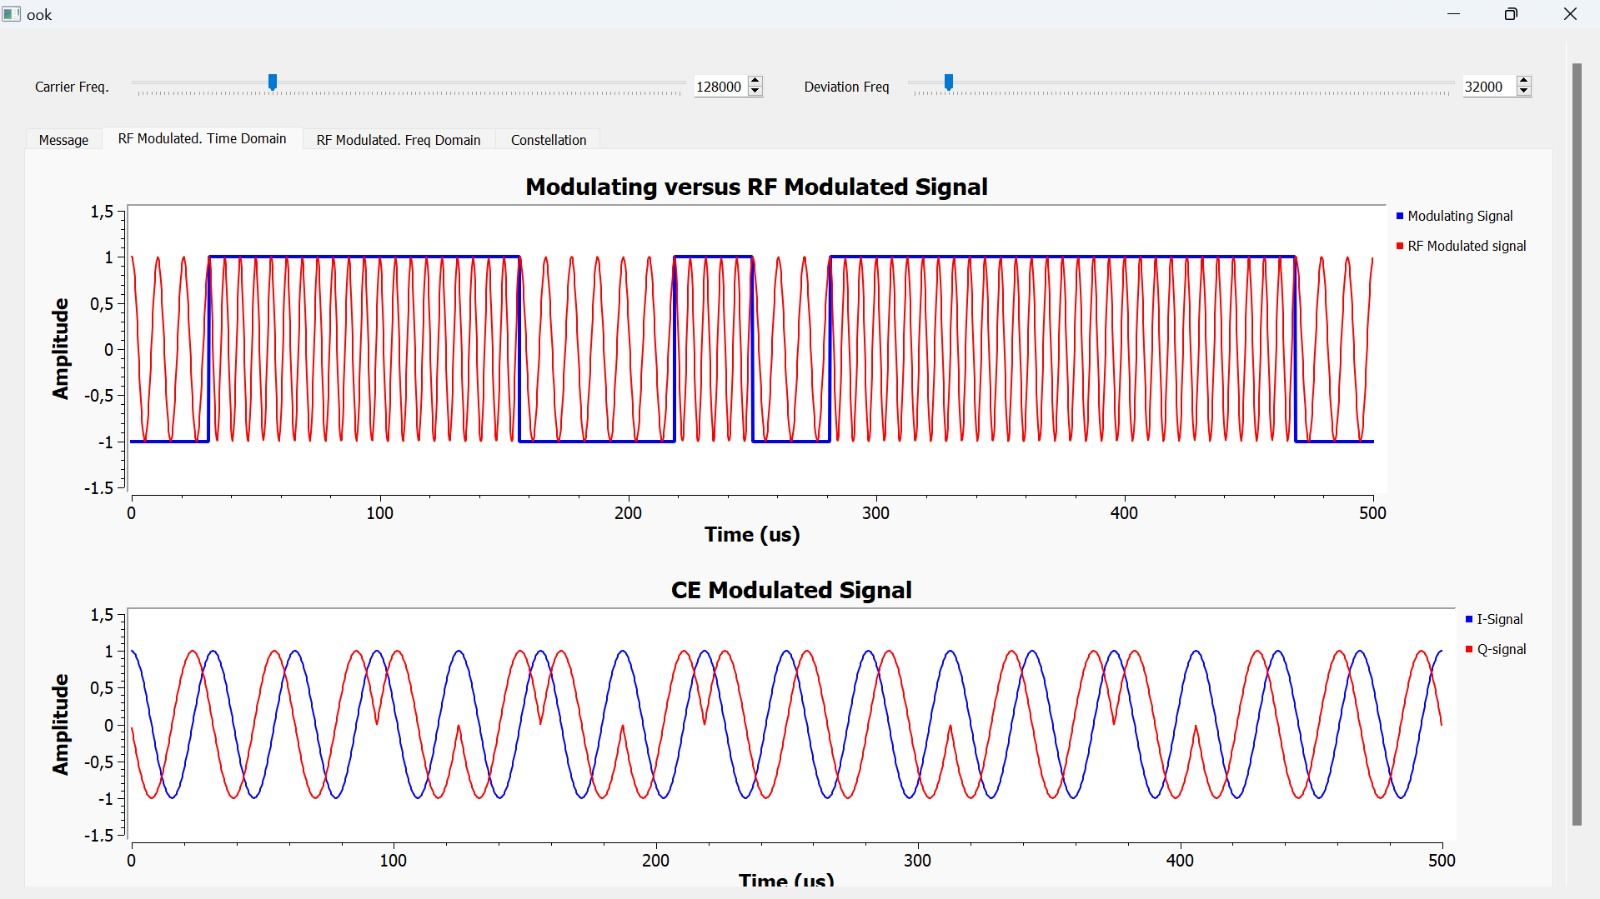
\includegraphics[width=0.45\textwidth]{figs/F7.png}
        \caption{Figura 7: Gráfica en tiempo RF y EC en fSK con frecuencias constantes}
        \label{fig:7}
    \end{center}
Mientras se observa el comportamiento de la señal modulada en versión RF y en versión EC en el dominio del tiempo (pestaña \texttt{Modulated-Time}):En la figura 8 La frecuencia de la portadora se varía a un valor de 323584 Hz, pero la desviación de frecuencias se mantiene constante.
 \begin{center}
        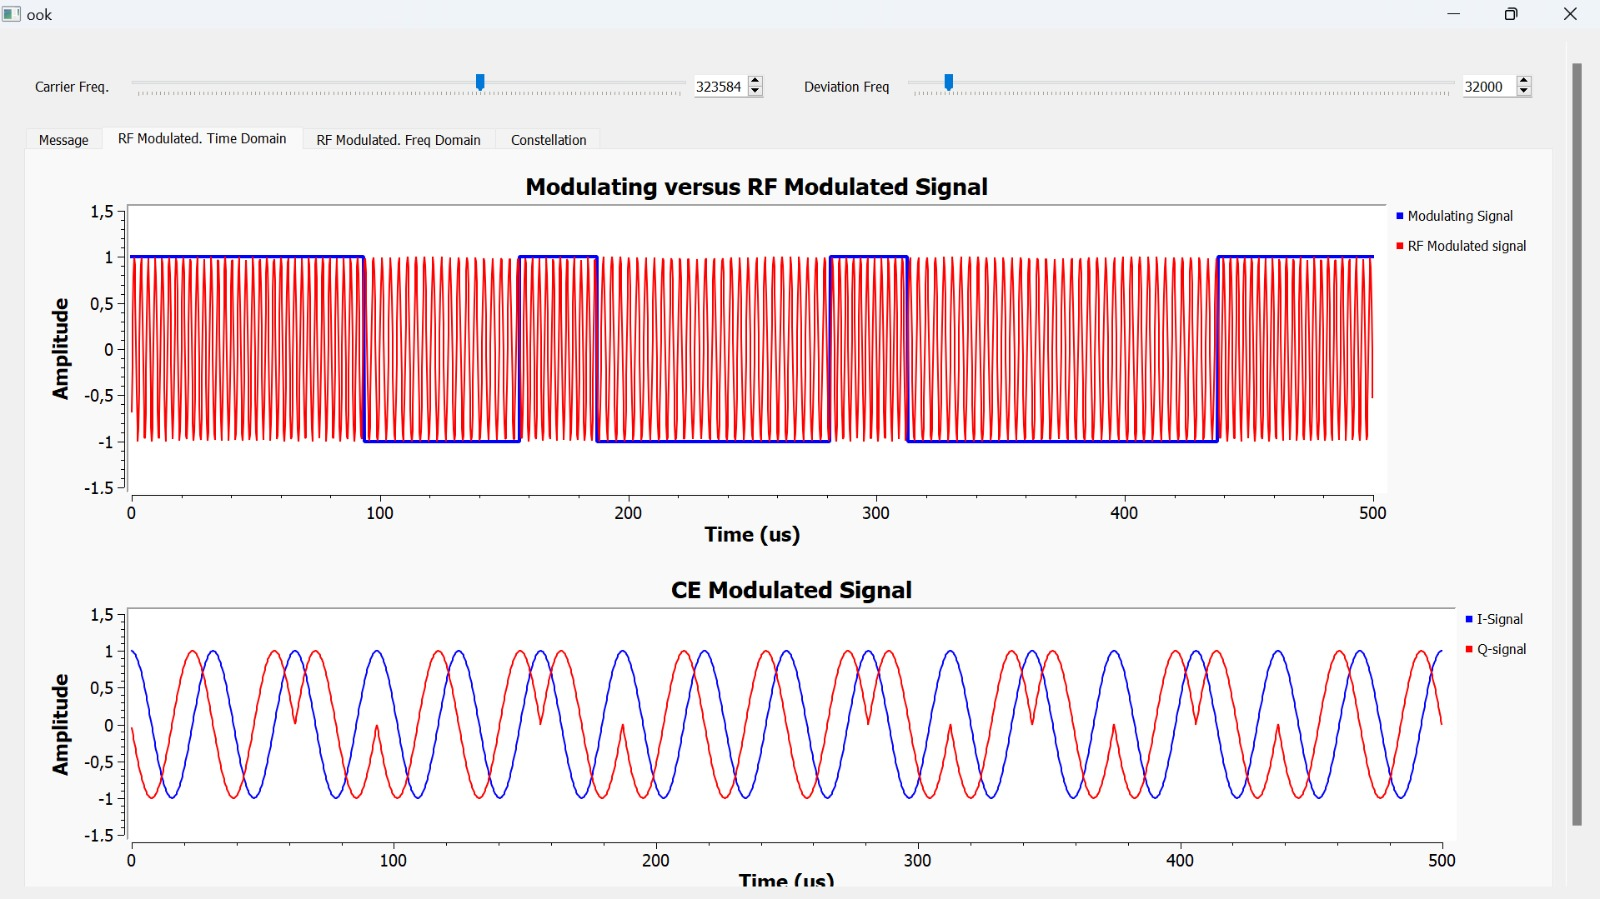
\includegraphics[width=0.45\textwidth]{figs/F8.png}
        \caption{Figura 8: Gráfica en tiempo RF y EC en fSK variando la frecuencia prtadora}
        \label{fig:8}
    \end{center}
Ahora en la figura 9 la frecuencia de la portadora se mantiene constante, pero se varía la desviación de frecuencias a un valor de 61440 Hz.
 \begin{center}
        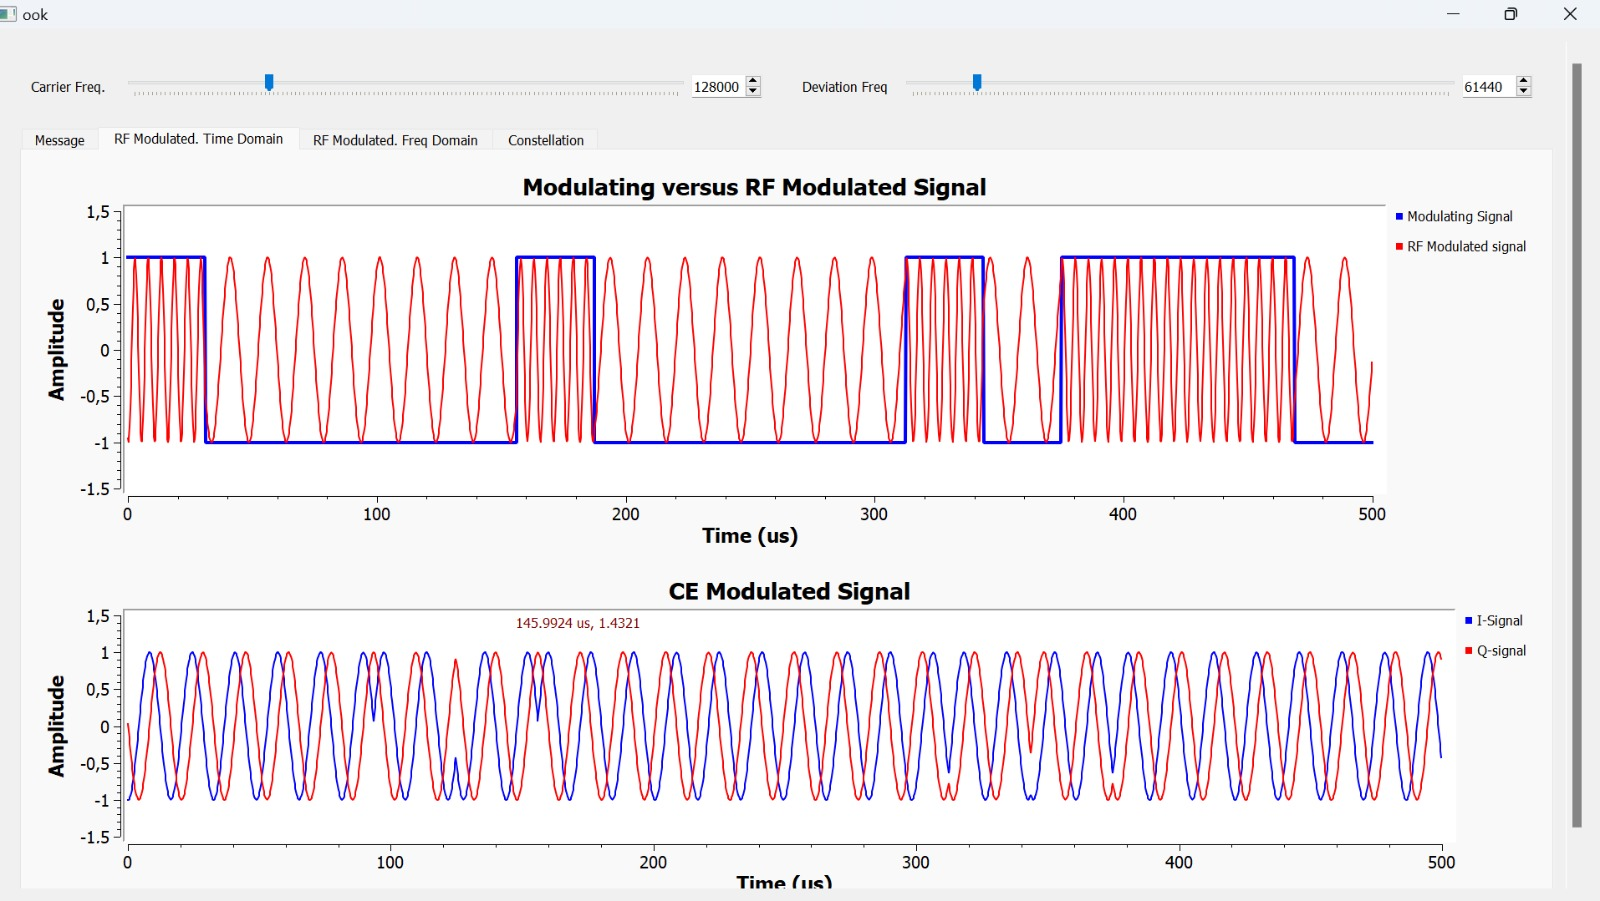
\includegraphics[width=0.45\textwidth]{figs/F9.png}
        \caption{Figura 9: Gráfica en tiempo RF y EC en fSK variando la desviacion de frecuancia}
        \label{fig:9}
    \end{center}
\paragraph{Observaciones de FSK en el dominio de las frecuencias}
En estas observaciones se trabaja con las mismas constantes y las mismas variaciones que en las observacionesde RF y EC, esta vez observando (pestaña Modulated-Freq)
En la figura 10 la frecuencia de la portadora se varía a un valor de 323584 Hz, pero la desviación de frecuencias se mantiene constante.
 \begin{center}
        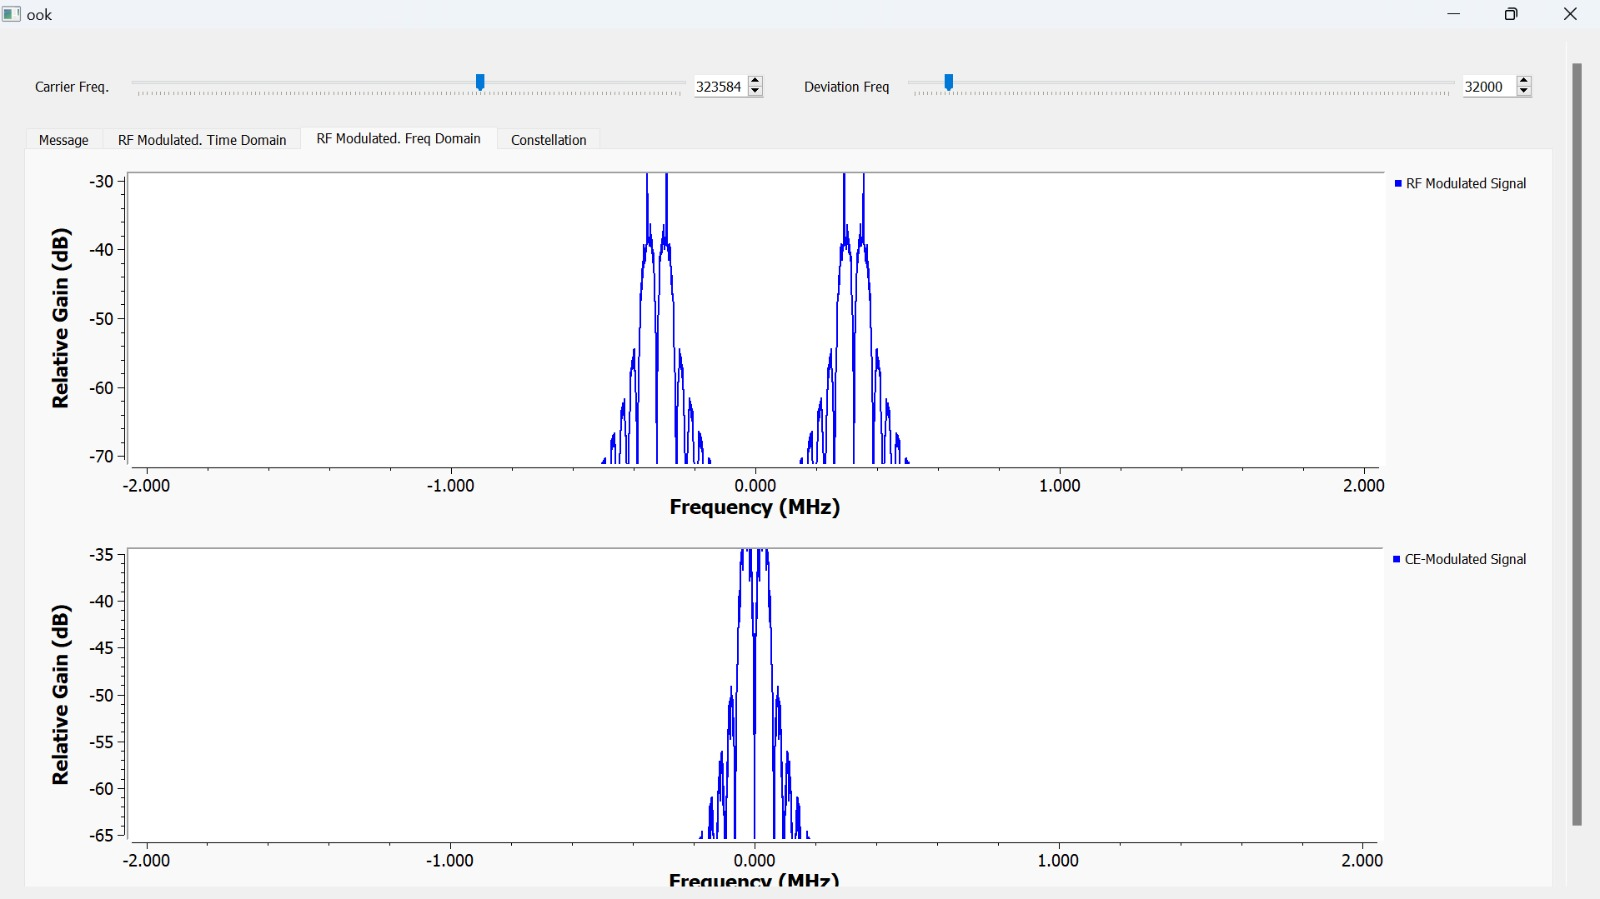
\includegraphics[width=0.45\textwidth]{figs/F10.png}
        \caption{Figura 10: Gráfica en frecuencias RF y EC en fSK variando la frecuancia portadora}
        \label{fig:10}
    \end{center}
 En la figura 11 la frecuencia de la portadora se mantiene constante, pero se varía la desviación de frecuencias a un valor de 61440 Hz.
 \begin{center}
        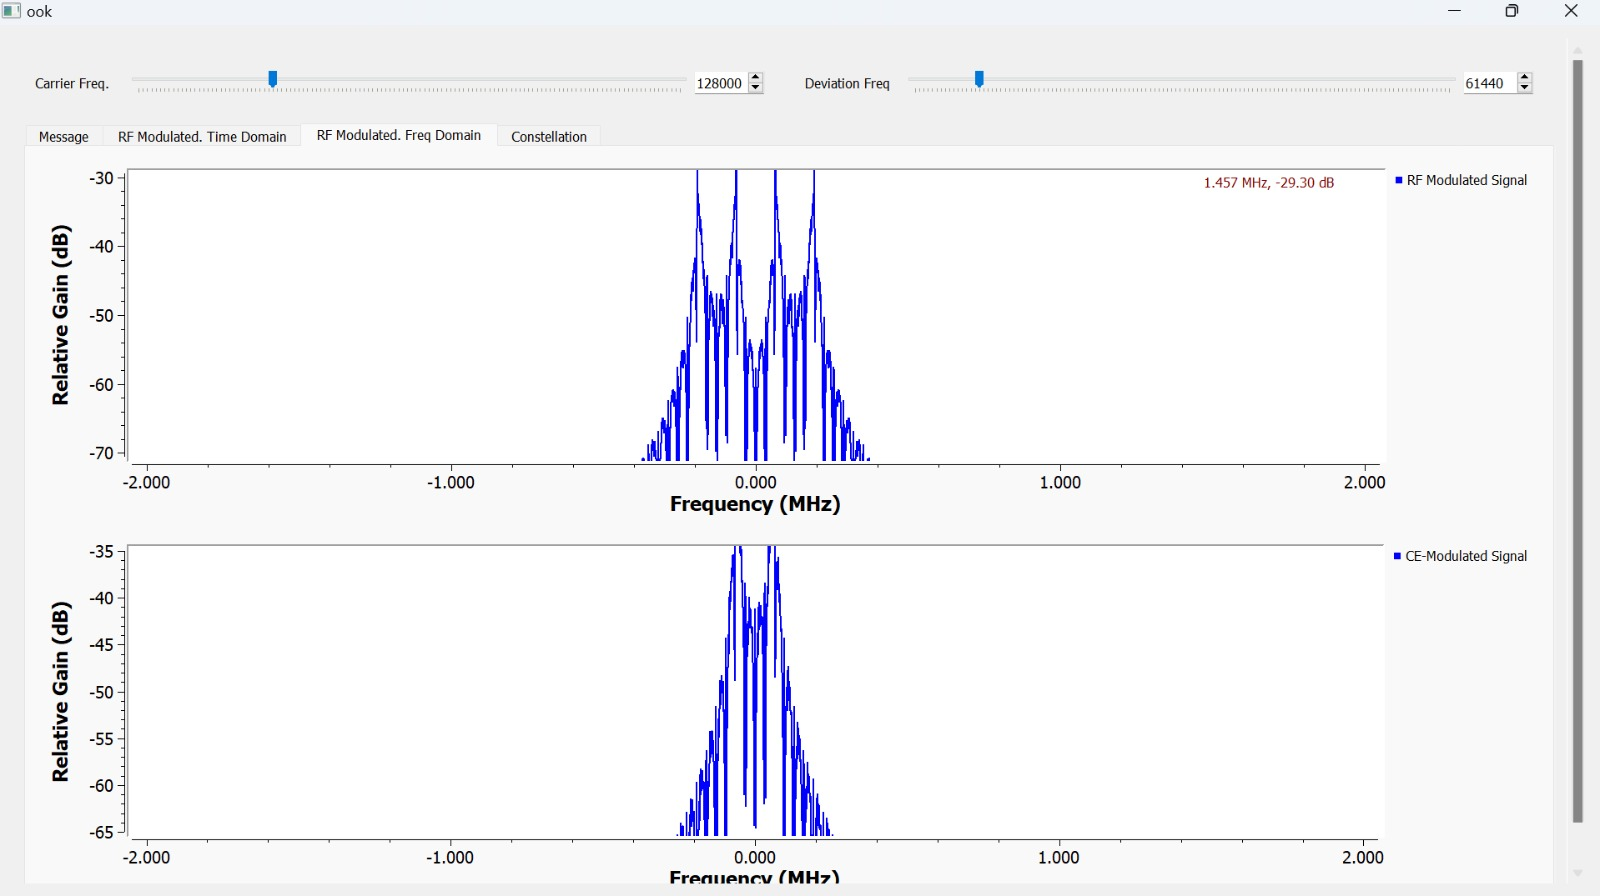
\includegraphics[width=0.45\textwidth]{figs/F11.png}
        \caption{Figura 11: Gráfica en frecuencias RF y EC en fSK variando la desviación de frecuencia}
        \label{fig:11}
    \end{center}
valor para la frecuencia portadora y para la desviación de 
frecuencias en el cual el espectro se puede distinguir con el menor solapamiento posible. 
Valores propuestos frecuencia portadora=512000 Hz, desviación de frecuencia=50000Hz

\paragraph{Observaciones de FSK en la Constelación}
En estas observaciones se trabaja con las mismas constantes y las mismas variaciones en (pestaña Constellation).
En la figura 12 la frecuencia de la portadora se varía a un valor de 323584 Hz, pero la desviación de frecuencias se mantiene constante.
 \begin{center}
        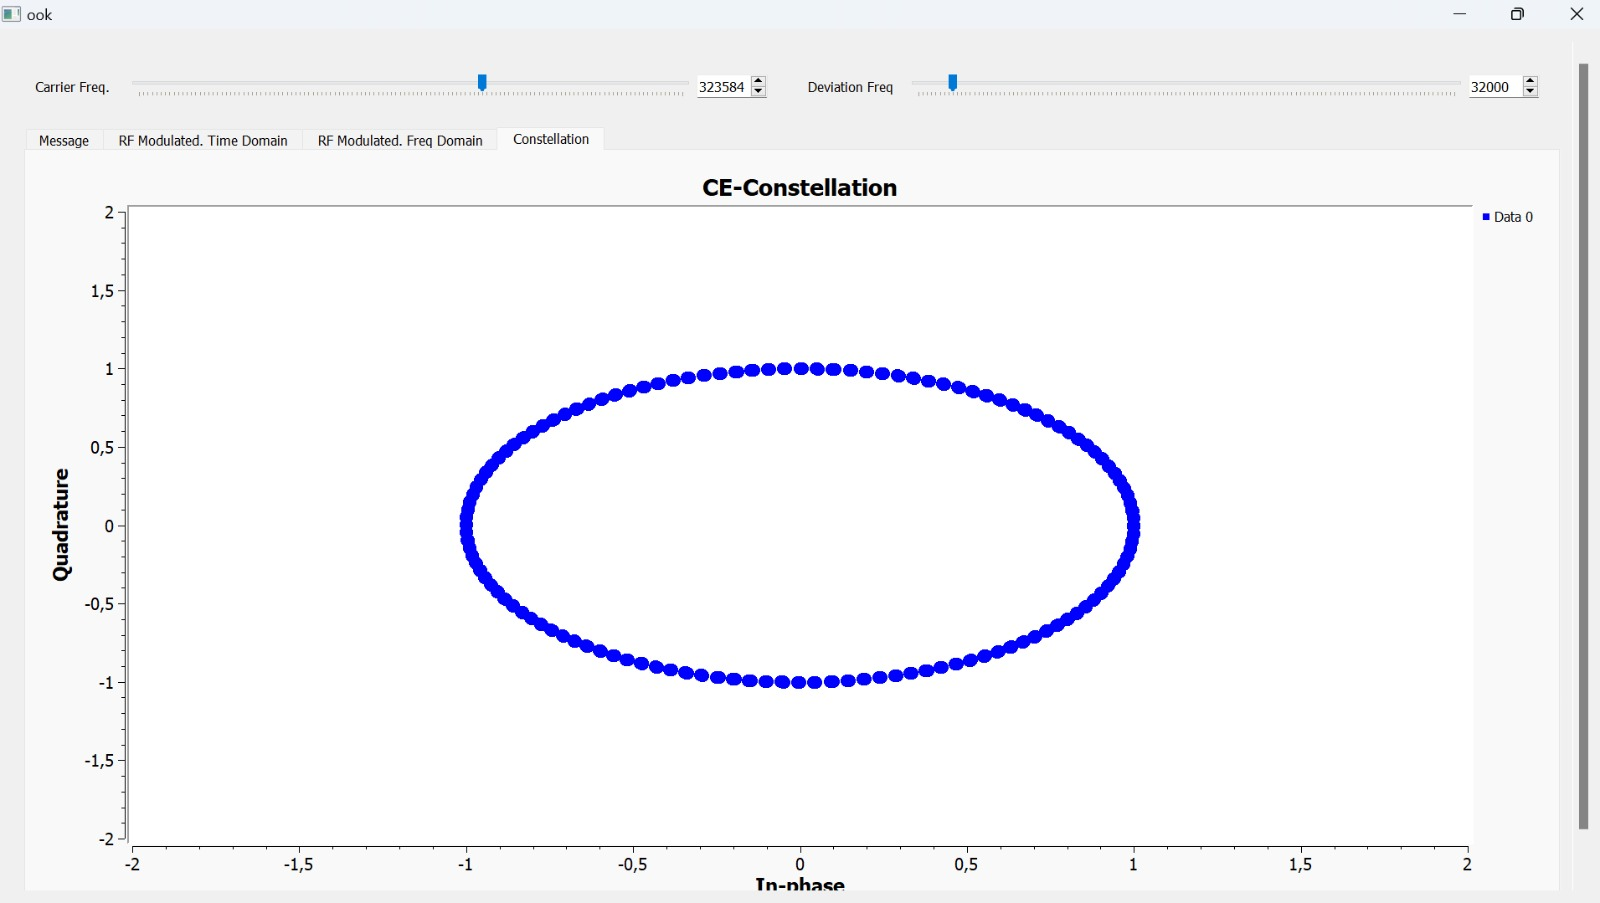
\includegraphics[width=0.45\textwidth]{figs/F12.png}
        \caption{Figura 12: Gráfica de constelaciones variando la frecuancia portadora}
        \label{fig:12}
    \end{center}
 En la figura 13 la frecuencia de la portadora se mantiene constante, pero se varía la desviación de frecuencias a un valor de 61440 Hz.
 \begin{center}
        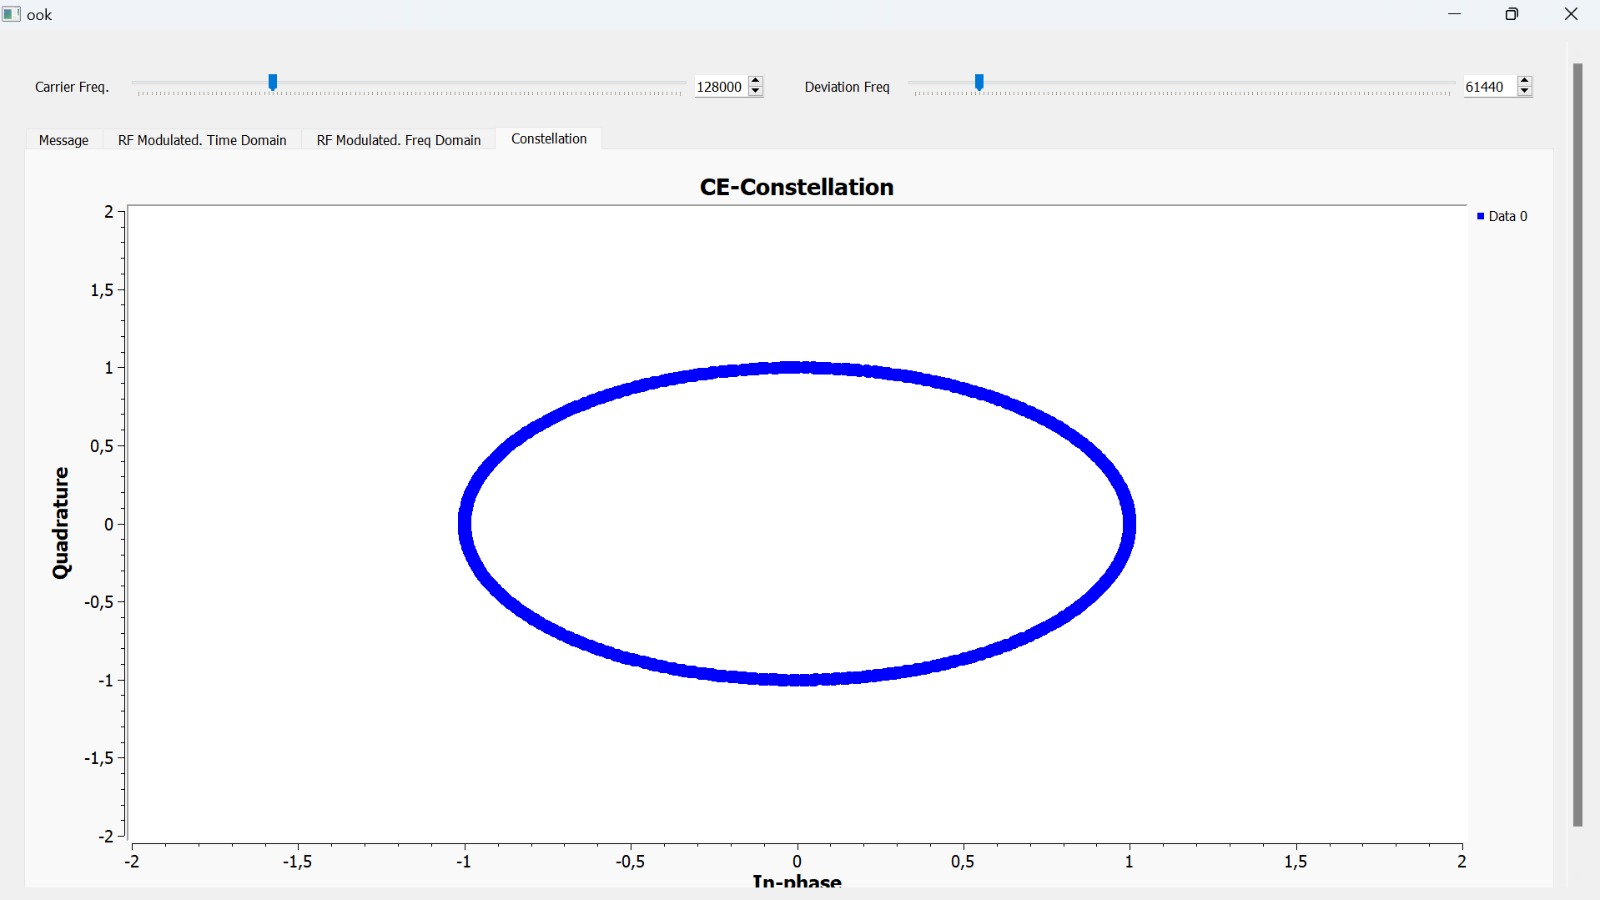
\includegraphics[width=0.45\textwidth]{figs/F16.png}
        \caption{Figura 13: Gráfica de constelaciones variando la desviación de frecuencia}
        \label{fig:13}
    \end{center}
Explique cómo es la constelación de una señal con modulación FSK.
El diagrama de constelación es una representación gráfica que ilustra los diferentes estados posibles de la señal modulada. En el caso de FSK:
una señal FSK no tiene una constelación en el sentido tradicional. 
Ejes del Diagrama: En lugar de representar las fases como en otras modulaciones (por ejemplo, PSK), los ejes del diagrama de constelación para FSK representan las frecuencias f1 y f2. Cada punto en el diagrama corresponde a un símbolo que representa una de las frecuencias utilizadas en la modulación.
Símbolos: Los símbolos en el diagrama no están dispuestos en un círculo como en PSK, sino que están ubicados a lo largo del eje horizontal (frecuencia) y vertical (amplitu). Esto significa que cada punto indica la frecuencia correspondiente a un símbolo específico.


\subsection{Parte E: Preguntas de control}

\section*{I.}
Para determinar si el valor de SPS elegido es apropiado, se debe considerar lo siguiente:

\begin{itemize}
    \item El valor de SPS debe ser suficientemente alto para evitar problemas de aliasing y asegurar una adecuada representación de la señal modulada en RF. Generalmente, se recomienda usar un valor de SPS al menos 4-8 veces mayor que el ancho de banda de la señal modulada.
    \item Un valor de SPS muy alto, aunque ayuda a reducir el aliasing, también aumenta la carga computacional. Se debe encontrar un equilibrio entre la calidad de la señal y los recursos disponibles.
    \item Para evaluar si el valor de SPS es apropiado, se puede analizar la señal modulada en el dominio de la frecuencia utilizando el bloque \texttt{qtgui\_freq\_sink\_x\_0}. Debe observarse una adecuada representación espectral sin problemas de aliasing.
\end{itemize}

\section*{II.}
Si el bloque \texttt{Multiply Const} se configura con un valor de 1, el resultado sería el mismo que quitarlo por completo. Esto se debe a que multiplicar por 1 no tiene ningún efecto sobre la señal.

\section*{III.}
La fórmula dentro del bloque \texttt{Multiply Const} para la modulación FSK sería:

\[
\text{Const} = \frac{2 \pi \cdot f_d}{R_b \cdot \text{SPS}}
\]

Donde:
\begin{itemize}
    \item $f_d$ es la desviación de frecuencia
    \item $R_b$ es la tasa de bits
    \item \text{SPS} es el número de muestras por símbolo
\end{itemize}

Esta fórmula calcula el factor de multiplicación necesario para desviar la frecuencia de la portadora de acuerdo a la señal modulante.

\section*{IV.}
El bloque \texttt{Constant Source} se configura a 0 para la modulación OOK porque en este caso la señal modulante simplemente enciende y apaga la portadora. No se requiere ninguna otra señal de entrada.

Para la modulación BPSK y FSK, la señal del bloque \texttt{Constant Source} se utiliza como la segunda entrada de los VCO, proporcionando la señal de fase o frecuencia que se modula.

\section*{V.}
En el caso de la modulación OOK, la señal modulante entra por la primera entrada de los VCO porque es la única entrada necesaria. Esta señal controla la amplitud de la portadora.

Para la modulación BPSK y FSK, la señal modulante entra por la segunda entrada de los VCO porque se utiliza para modular la fase o frecuencia de la portadora, mientras que la primera entrada se reserva para una señal de amplitud constante.

\section*{VI-VII.}
Sí, sería posible reubicar el bloque \texttt{Interpolating FIR Filter} para que quede inmediatamente antes de los VCO tanto en la modulación BPSK como en la FSK. Esto no cambiaría el funcionamiento del sistema, sino que simplemente modificaría la ubicación del filtro en el diagrama de bloques.


\section*{a.}
Para crear un VCO RF con entradas de amplitud y frecuencia, usaría los siguientes bloques de GNU Radio:

\begin{itemize}
    \item \texttt{epy\_block} para el VCO RF en sí, tomando las señales de amplitud y frecuencia como entradas y generando la señal RF modulada como salida.
    \item \texttt{qtgui\_time\_sink\_x} y \texttt{qtgui\_freq\_sink\_x} para visualizar las señales moduladoras y la salida RF en el dominio del tiempo y la frecuencia.
\end{itemize}

Los aspectos clave serían:
\begin{itemize}
    \item Implementar la funcionalidad del VCO RF en el \texttt{epy\_block} personalizado, convirtiendo las entradas de amplitud y frecuencia en una señal RF.
    \item Conectar las señales moduladoras de amplitud y frecuencia a las entradas del \texttt{epy\_block}.
    \item Usar los bloques de visualización para mostrar las señales en varios puntos del flujo.
\end{itemize}

\section*{b.}
Para el caso FSK dado, la máxima frecuencia de portadora $f_c$ permitida sería:

\[
f_{c_{\text{max}}} = \frac{R_b \cdot S_{ps}}{8}
\]

Donde:
\begin{itemize}
    \item $R_b$ es la tasa de bits (32000)
    \item $S_{ps}$ es el número de muestras por símbolo (128)
\end{itemize}

Sustituyendo los valores:

\[
f_{c_{\text{max}}} = \frac{32000 \cdot 128}{8} = 512000 \, \text{Hz}
\]

Por lo tanto, la máxima frecuencia de portadora permitida sería 512 kHz.

\section*{c.}
Para el caso FSK dado, la máxima desviación de frecuencia $f_d$ permitida sería:

\[
f_{d_{\text{max}}} = \frac{R_b}{2}
\]

Donde:
\begin{itemize}
    \item $R_b$ es la tasa de bits (32000)
\end{itemize}

Sustituyendo el valor:

\[
f_{d_{\text{max}}} = \frac{32000}{2} = 16000 \, \text{Hz}
\]

Por lo tanto, la máxima desviación de frecuencia permitida sería 16 kHz.

\section*{d.}
Para el caso BPSK dado, el mínimo valor de SPS (muestras por símbolo) sería:

\[
SPS_{\text{min}} = 2
\]

Este es el mínimo requerido para representar adecuadamente la señal modulada en BPSK y reconstruir los bits originales.

\section{Conclusiones}

\begin{itemize}
    
    \item Se lograron identificar las principales diferencias entre las modulaciones RF y EC a través de las señales generadas y analizadas en GNURadio. En la modulación RF, las señales se procesaron directamente en alta frecuencia, mientras que en EC se separaron en las componentes I (real) y Q (imaginaria), lo que permitió un análisis más detallado y adaptable en sistemas digitales.
    
    \item En el dominio del tiempo, cada modulación presentó características específicas. Por ejemplo, la modulación FSK mostró transiciones de frecuencia, mientras que BPSK y OOK destacaron por sus cambios abruptos en fase o encendido/apagado de la portadora, respectivamente.
    
    \item En las modulaciones EC, las señales moduladas se descomponen en I y Q, permitiendo procesarlas más fácil en sistemas digitales y simplifica la demodulación. En cambio, las modulaciones RF trabajan directamente con la señal portadora, lo que requiere más directo, pero menos versátil para sistemas modernos.
    
    \item Las simulaciones y análisis evidenciaron cómo los principios teóricos de la modulación digital se aplican en sistemas reales, permitiendo comprender las características y limitaciones de cada técnica para su implementación en aplicaciones prácticas.
     
    
\end{itemize}

\begin{thebibliography}{1}

\bibitem{flujgrama}
"Flujograma del proyecto en GNURadio", [En línea]: \url{https://github.com/hortegab/ComdigPractices2021sii/blob/main/Fase%20I/Pract4/RF_EC_ook.grc}.

\bibitem{OOK}
"Modulación On-Off Keying (OOK)," [En línea]: \url{https://n9.cl/pekzh}.

\bibitem{libro1} 
H. Ortega y R. Reyes, *Comunicaciones Digitales Basadas en Radio Definida por Software*. Capítulo 5, (UIS), 2019.


\end{thebibliography}

\end{multicols}

\end{document}
